\begin{document}
\renewcommand{\thefigure}{SI.\arabic{figure}}
\setcounter{figure}{0}

\renewcommand{\thetable}{SI.\arabic{table}}
\setcounter{table}{0}

\section*{Supplementary Information}\label{sec:SI}

\addcontentsline{toc}{section}{Supplementary Information}
\addtocontents{toc}{\setcounter{tocdepth}{-10}}
\renewcommand{\thesubsection}{SI.\arabic{subsection}}
\setcounter{subsection}{0}


\subsection{Overview of EMP Dataset Information}

\begin{figure}[H]
    \centering
    \includegraphics[scale=0.9]{./Figures/Chao_T_all}
    \caption{\textbf{The relationship between Chao1 index and temperature.} Bacterial diversity decreases with increasing temperature.}
    \label{fig:Chao_T}
\end{figure}

\begin{figure}[H]
    \centering
    \includegraphics[scale=0.9]{./Figures/OO_T_all}
    \caption{\textbf{The relationship between observed OTUs and temperature.} Bacterial diversity decreases with increasing temperature.}
    \label{fig:OO_T}
\end{figure}

\begin{figure}[H]
    \centering
    \includegraphics[scale=0.9]{./Figures/Shan_T_all}
    \caption{\textbf{The relationship between Shannon index and temperature.} Bacterial diversity decreases with increasing temperature.}
    \label{fig:Shan_T}
\end{figure}

\begin{figure}[H]
    \centering
    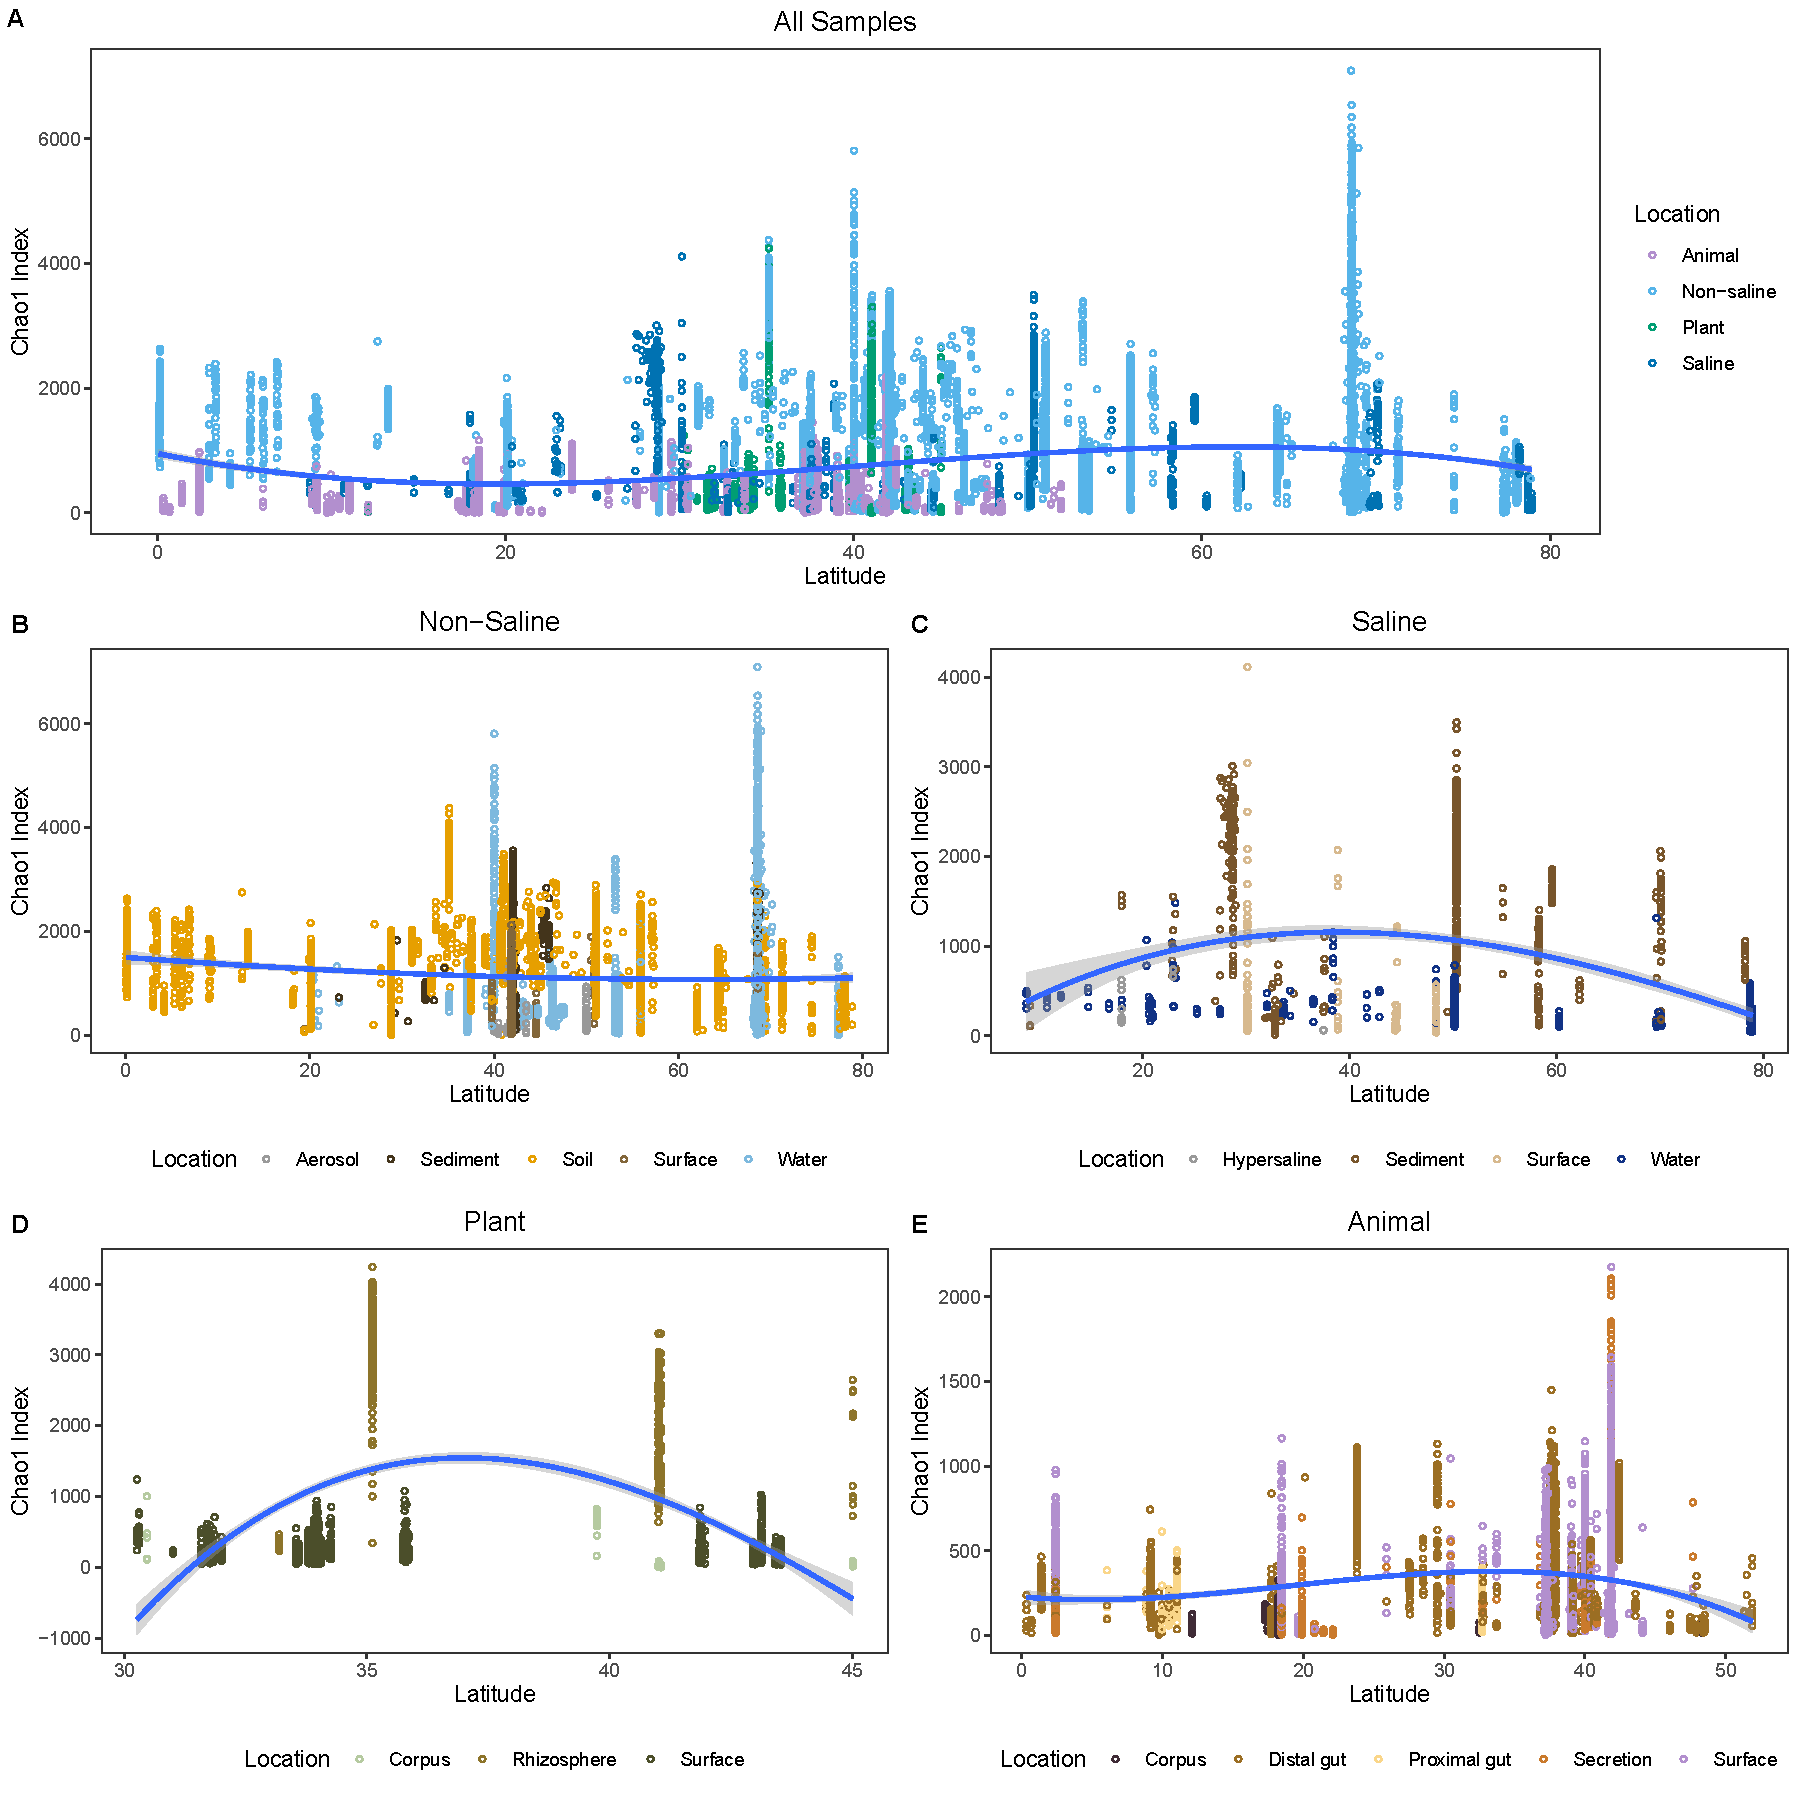
\includegraphics[scale=0.9]{./Figures/Chao_lati_empo2}
    \caption{\textbf{The relationship between Chao1 index and latitude.} A: Trend of Chao1 index with latitude for the whole data set. B: Chao1 index decreases with increasing latitude for non-saline samples. C-E: Chao1 index peaks at mid-latitude in saline, plant and animal data sets.}
    \label{fig:Chao_lati}
\end{figure}

\begin{figure}[H]
    \centering
    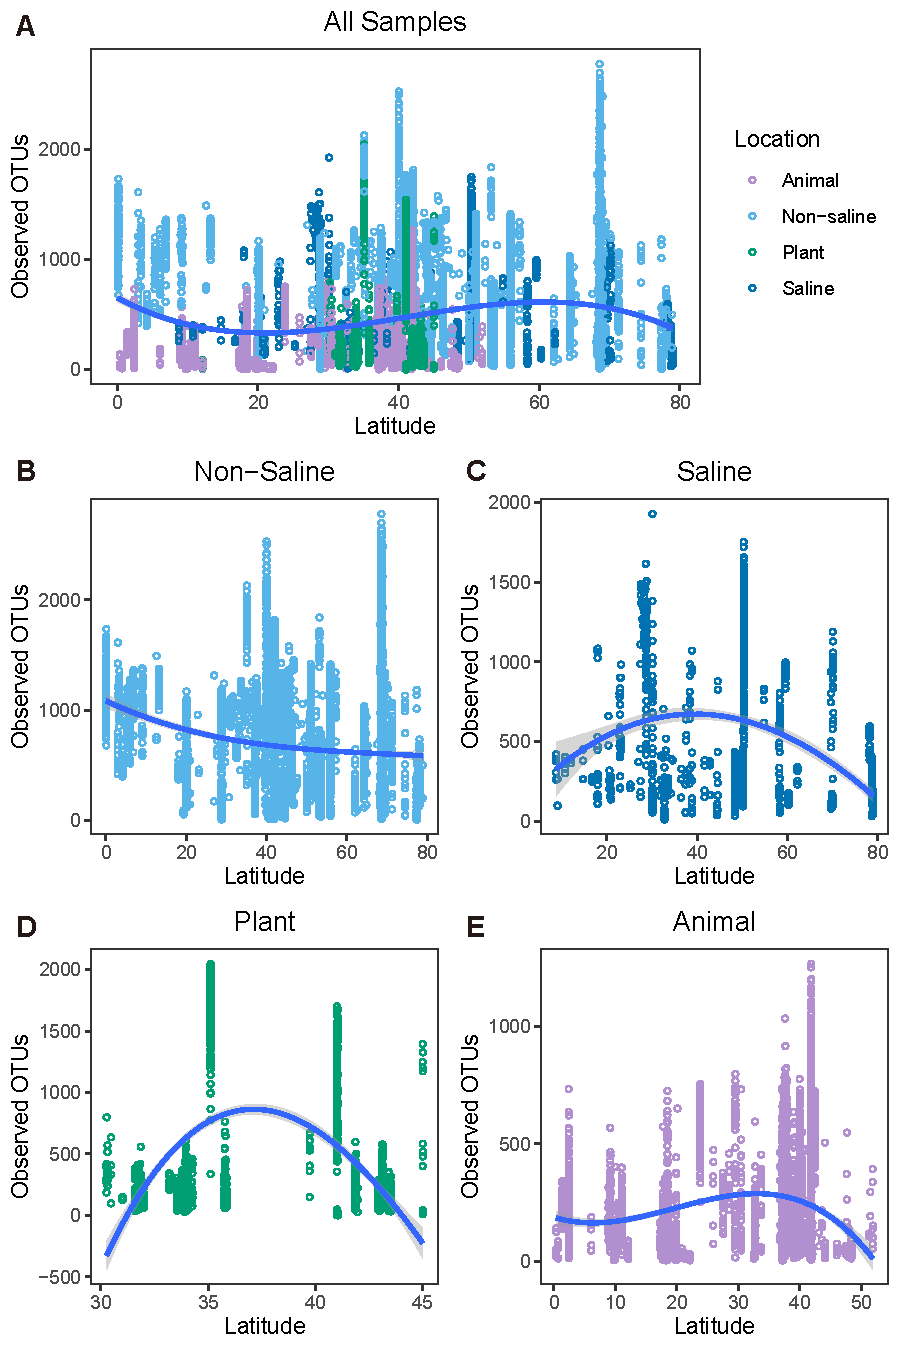
\includegraphics[scale=0.9]{./Figures/OO_lati_empo2}
    \caption{\textbf{The relationship between observed OTUs and latitude.} A: Trend of observed OTUs with latitude for the whole data set. B: Observed OTUs decreases with increasing latitude for non-saline samples. C-E: Observed OTUs peaks at mid-latitude in saline, plant and animal data sets.}
    \label{fig:OO_lati}
\end{figure}

\begin{figure}[H]
    \centering
    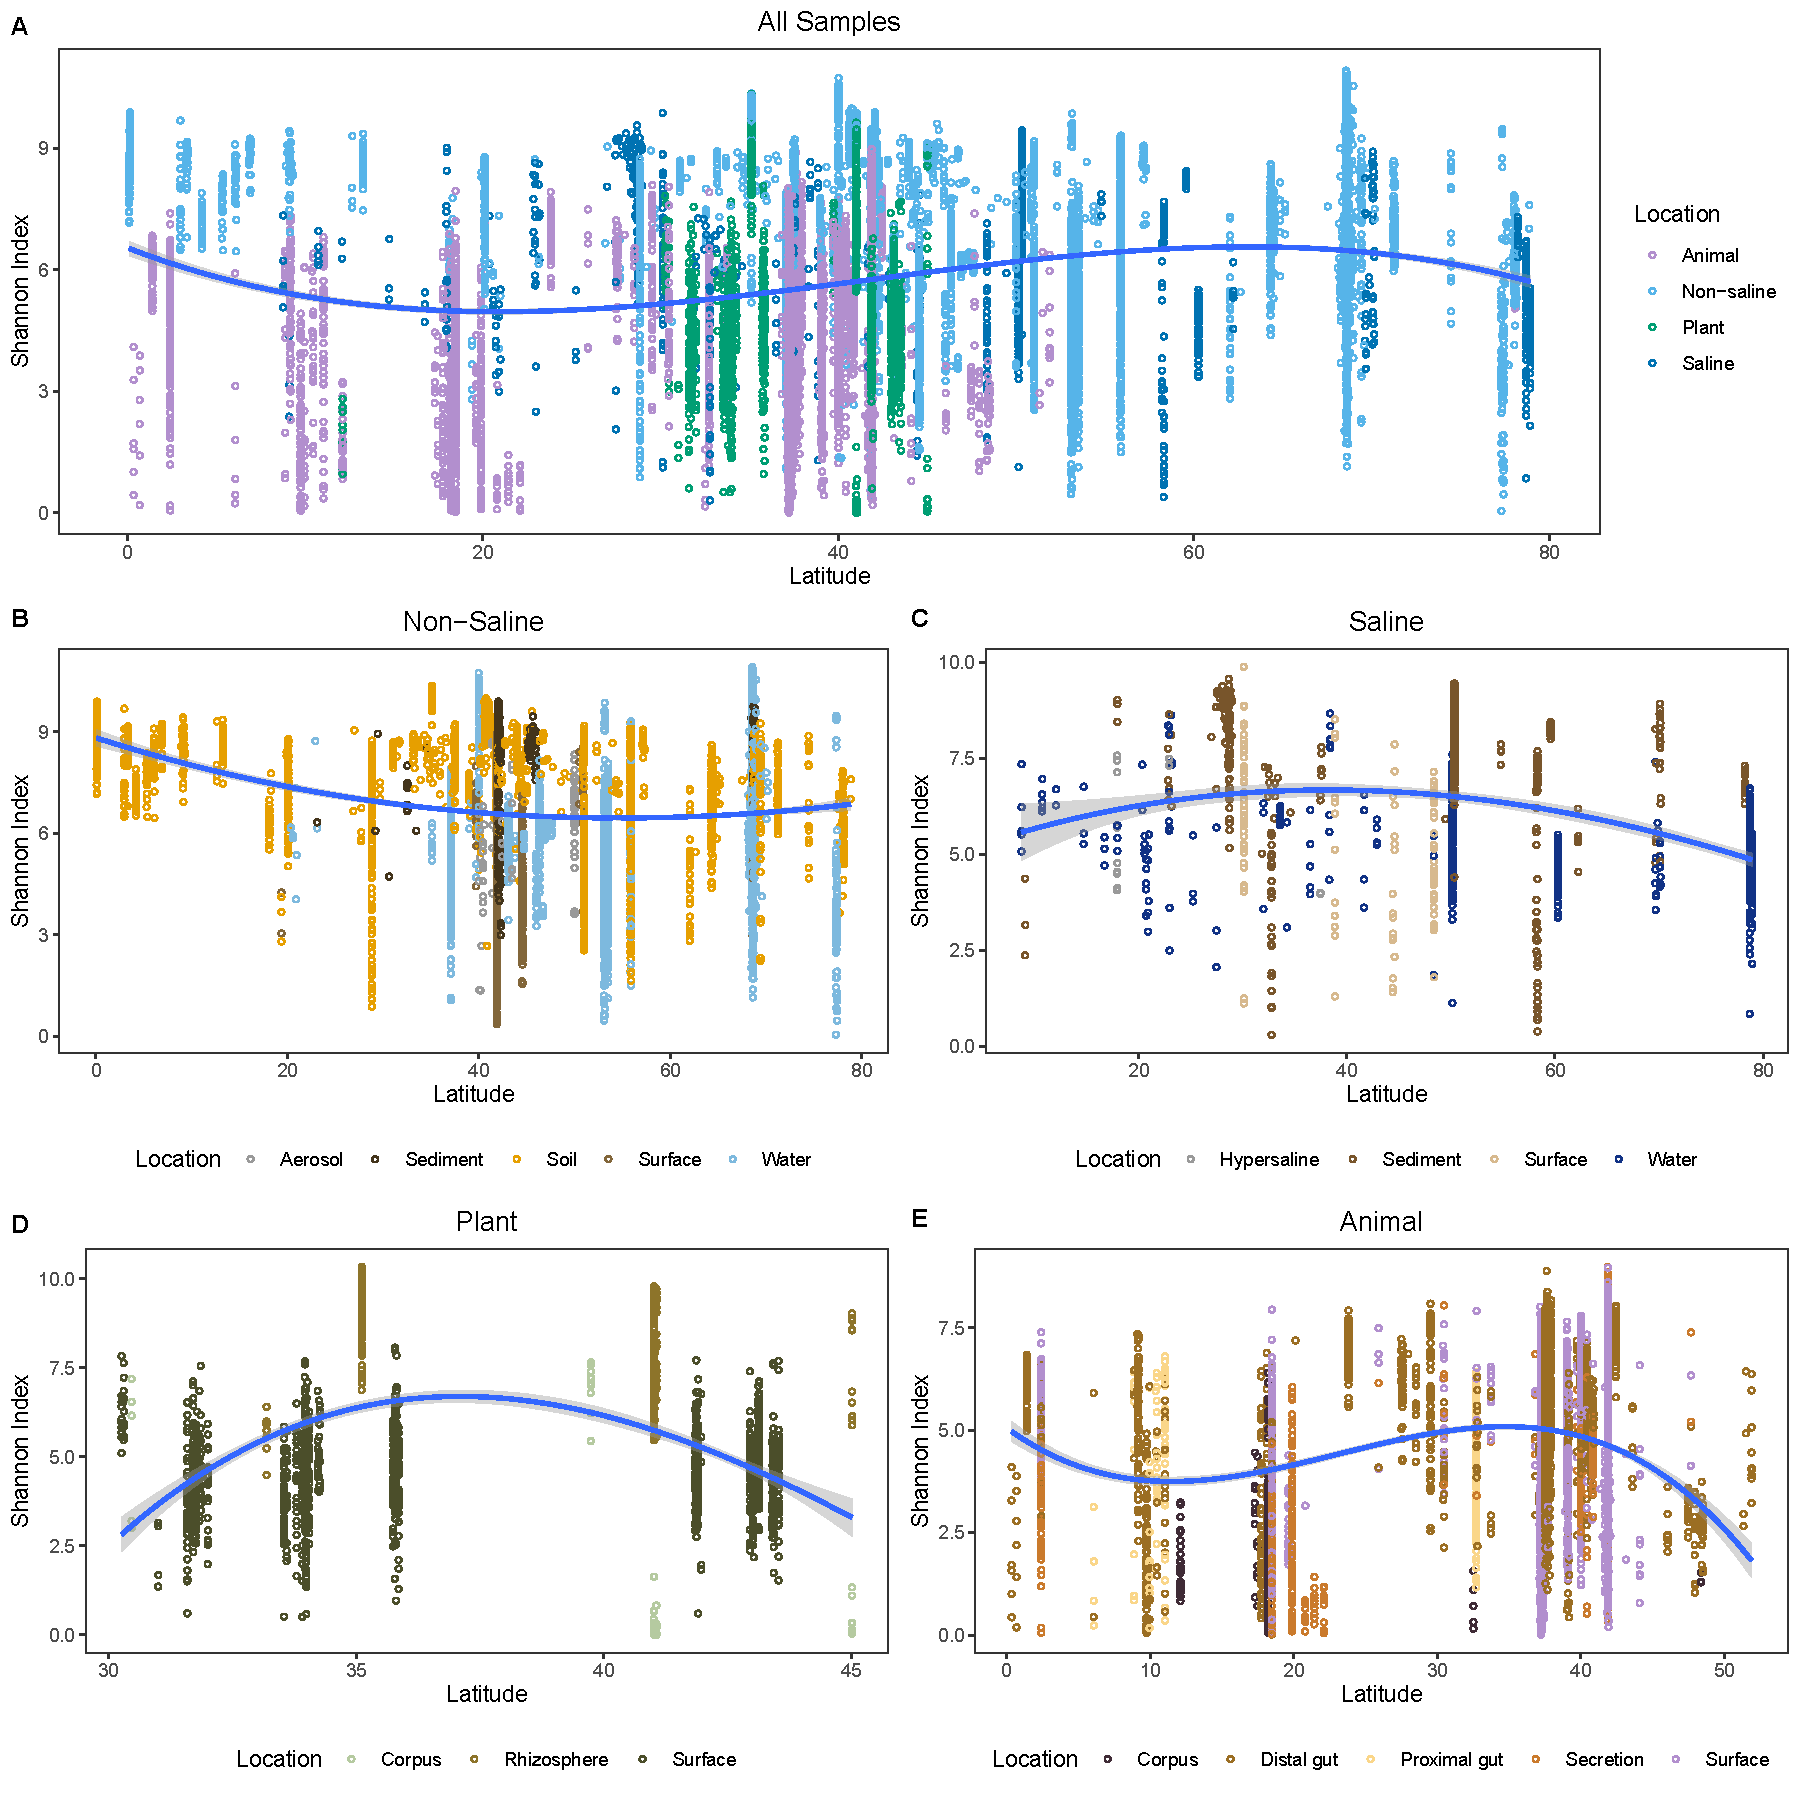
\includegraphics[scale=0.9]{./Figures/Shan_lati_empo2}
    \caption{\textbf{The relationship between Shannon index and latitude.} A: Trend of Shannon index with latitude for the whole data set. B: Shannon index decreases with increasing latitude for non-saline samples. C-E: Shannon index peaks at mid-latitude in saline, plant and animal data sets.}
    \label{fig:Shan_lati}
\end{figure}

\begin{figure}[H]
    \centering
    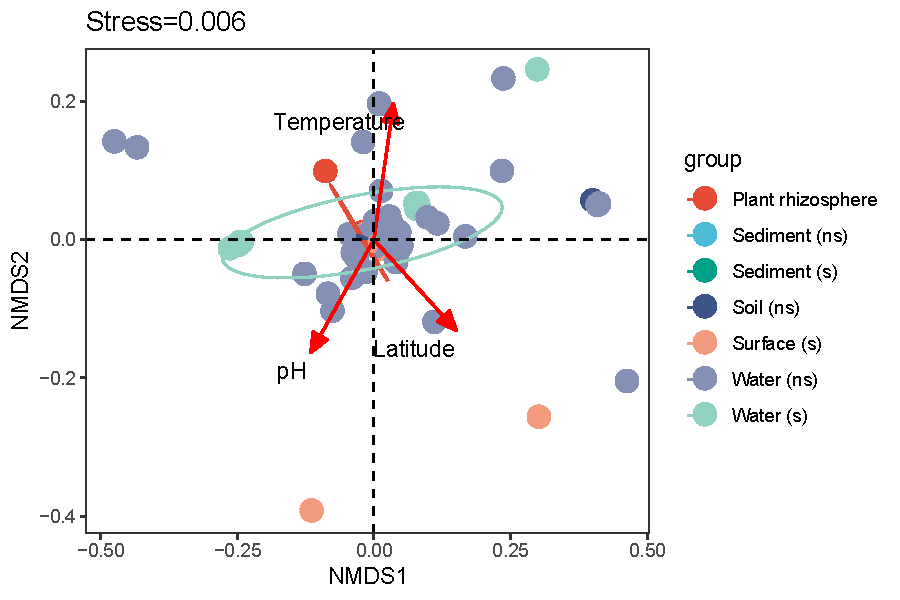
\includegraphics[scale=1]{./Figures/nmds_envfit_empo3}
    \caption{\textbf{Non-metric multidimensional scaling (NMDS) analysis of Bray-Curtis dissimilarity showing bacterial communities composition of filtered data set.} The figure shows that the differences in community composition are not significant, where "ns" stands for "non-saline" and "s" for "saline".}
    \label{fig:nmds}
\end{figure}

\subsection{The relationships between bacterial diversity and environmental variables}

\begin{figure}[H]
    \centering
    \includegraphics[scale=0.15]{./Figures/PairsPlot}
    \caption{\textbf{The relationship between diversity indices, temperature, pH and latitude.} A: The relationship between Chao1 index, temperature, pH and latitude. B: The relationship between observed OTUs, temperature, pH and latitude. C: The relationship between Shannon index, temperature, pH and latitude..}
    \label{fig:Pairs}
\end{figure}

\begin{table}[H]
    \caption{{\bf The performance of polynomial and random forest in determining the effect of environmental variables on bacterial community diversity.} The interaction effect of the three environmental variables is the most influential factor on diversity in all models. Latitude performs best of the three environmental variables.} 
     \centering
    \begin{tabular}{ m{4cm}<{\centering}m{0.9cm}<{\centering}m{4cm}<{\centering}m{4cm}<{\centering}} 
    \toprule
     Diversity & $R^{2}$ & Polynomial Model & Random Forest Model \\
     \midrule
    \multirow{7}*{Chao1 Richness} & T*p*L & 0.131 & 0.423 \\
    & T*p & 0.072 & 0.171 \\
    & T*L & 0.118 & 0.456 \\
    & p*L & 0.107 & 0.454 \\
    & T & 0.044 & 0.078 \\
    & p & 0.053 & 0.118 \\
    & L & 0.1 & 0.49 \\
     \midrule
    \multirow{7}*{Absolute Richness} & T*p*L & 0.127 & 0.437 \\
    & T*p & 0.076 & 0.179 \\
    & T*L & 0.114 & 0.47 \\
    & p*L & 0.092 & 0.456 \\
    & T & 0.052 & 0.083 \\
    & p & 0.048 & 0.116 \\
    & L & 0.083 & 0.496 \\
     \midrule
    \multirow{7}*{Phylogenetic Diversity} & T*p*L & 0.207 & 0.422 \\
    & T*p & 0.048 & 0.235 \\
    & T*L & 0.128 & 0.436 \\
    & p*L & 0.139 & 0.419 \\
    & T & 0.018 & 0.018 \\
    & p & 0.017 & 0.127 \\
    & L & 0.092 & 0.462 \\
    \bottomrule
    \end{tabular}    
    \label{tab:models}
\end{table}

\begin{figure}[H]
    \centering
    \includegraphics[scale=0.8]{./Figures/Chao_PM_simpleTpL}
    \caption{\textbf{Effect of a single environmental variables on Chao1 richness at the global scale.} A-C: Polynomial regression models of richness and temperature, pH and latitude ($R^{2}$=0.044, 0.053, 0.1). Chao1 richness peaks at around 6.3 \textdegree C and pH around 6.6. Latitude performs best in these models.}
    \label{fig:Chao_PM_simpleTpL}
\end{figure}

\begin{figure}[H]
    \centering
    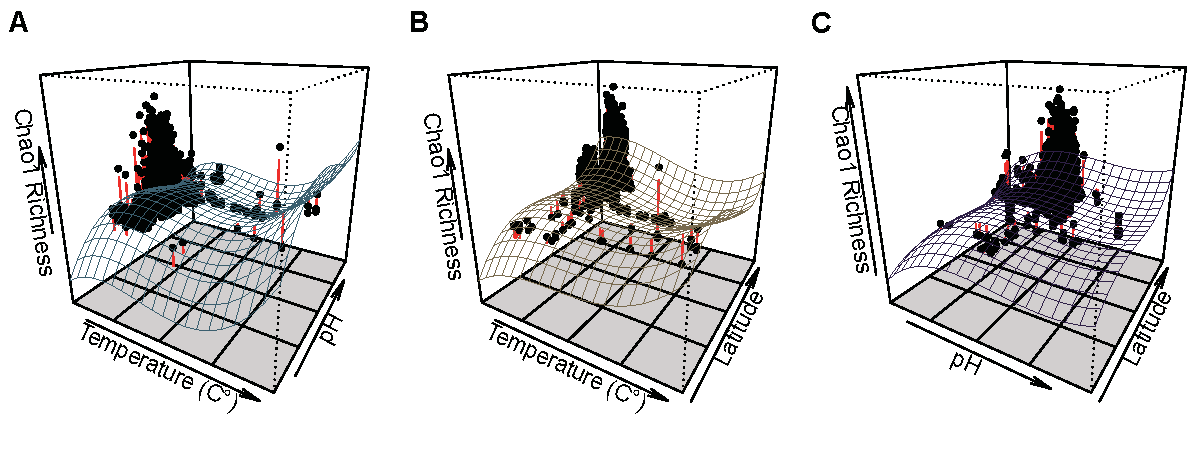
\includegraphics[scale=0.8]{./Figures/Chao_PM_all_2EVs_3D}
    \caption{\textbf{Effect of two environmental variables on Chao1 richness at the global scale.} A: Polynomial regression model of Chao1 richness versus temperature and pH ($R^{2}$=0.072). B: Model of richness versus temperature and latitude ($R^{2}$=0.118). C: Model of richness versus pH and latitude ($R^{2}$=0.107).}
    \label{fig:Chao_PM_2EVs}
\end{figure}

\begin{figure}[H]
    \centering
    \includegraphics[scale=0.8]{./Figures/OO_PM_simpleTpL}
    \caption{\textbf{Effect of a single environmental variables on absolute species richness (observed OTUs) at the global scale.} A-C: Polynomial regression models of richness and temperature, pH and latitude ($R^{2}$=0.052, 0.048, 0.083). Chao1 richness peaks at around 6.3 \textdegree C and pH around 6.6. Latitude performs best in these models.}
    \label{fig:OO_PM_simpleTpL}
\end{figure}

\begin{figure}[H]
    \centering
    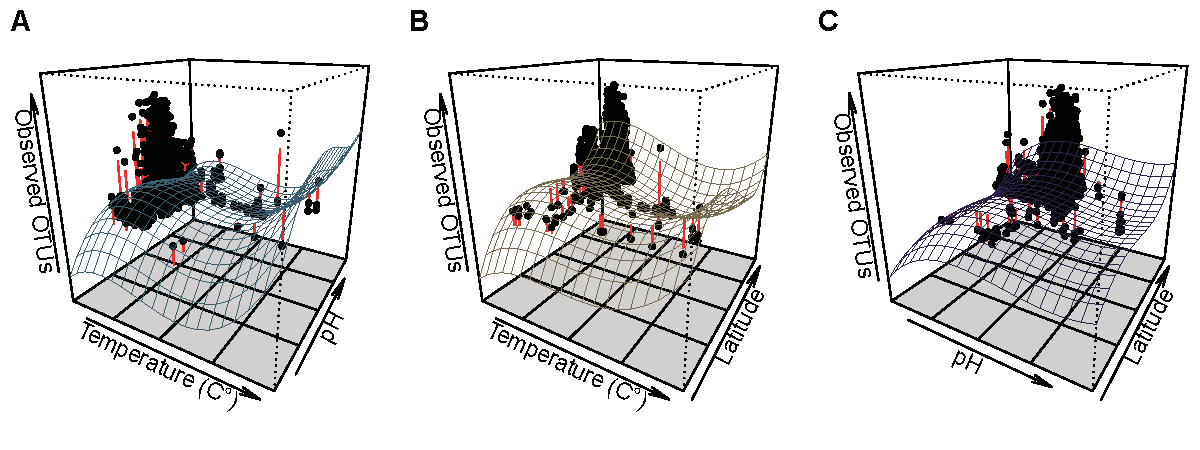
\includegraphics[scale=0.8]{./Figures/OO_PM_all_2EVs_3D}
    \caption{\textbf{Effect of two environmental variables on absolute species richness (observed OTUs) at the global scale.} A: Polynomial regression model of richness versus temperature and pH ($R^{2}$=0.076). B: Model of richness versus temperature and latitude ($R^{2}$=0.114). C: Model of richness versus pH and latitude ($R^{2}$=0.092).}
    \label{fig:OO_PM_2EVs}
\end{figure}

\begin{figure}[H]
    \centering
    \includegraphics[scale=0.8]{./Figures/PD_PM_simpleTpL}
    \caption{\textbf{Effect of a single environmental variables on phylogenetic diversity at the global scale.} A-C: Polynomial regression models of phylogenetic diversity and temperature, pH and latitude ($R^{2}$=0.018, 0.017, 0.092). Latitude performs best in these models. }
    \label{fig:PD_PM_simpleTpL}
\end{figure}

\begin{figure}[H]
    \centering
    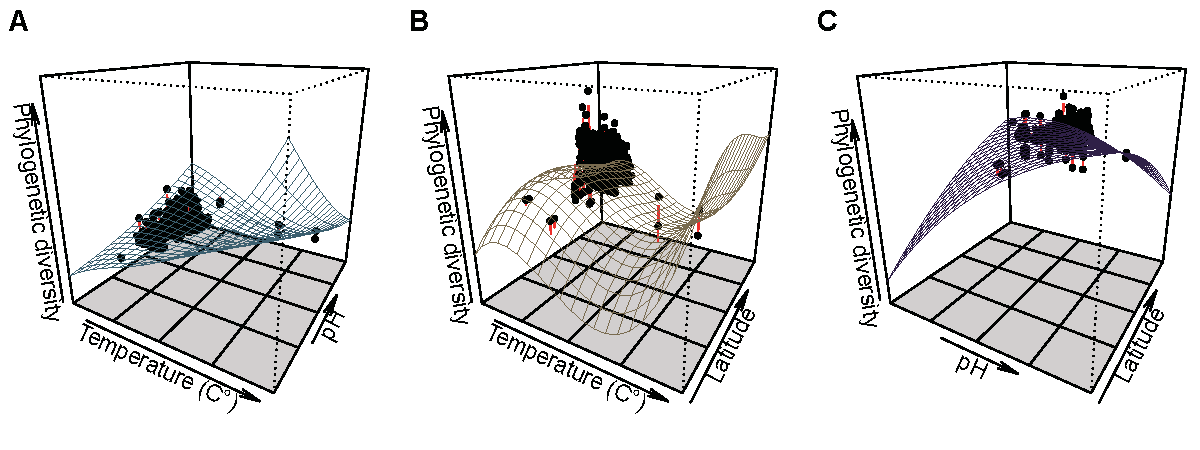
\includegraphics[scale=0.8]{./Figures/PD_PM_all_2EVs_3D}
    \caption{\textbf{Effect of temperature and pH on phylogenetic diversity at the global scale.} A: Polynomial regression model of phylogenetic diversity versus temperature and pH ($R^{2}$=0.0483). B: Model of diversity versus temperature and latitude ($R^{2}$=0.128). C: Model of diversity versus pH and latitude ($R^{2}$=0.139).}
    \label{fig:PD_PM_2EVs}
\end{figure}

\begin{table}[H]
    \caption{{\bf R-square of the EMPO3 models between Chao1 richness, absolute richness (observed OTUs) and Shannon diversity and environmental variables.}PM and RF are polynomial regression models and random forest models respectively.}
    \centering
    \begin{tabular}{ m{4cm}<{\centering}m{0.9cm}<{\centering}m{2cm}<{\centering}m{2cm}<{\centering}m{2cm}<{\centering}m{2cm}<{\centering}} 
    \toprule
     Environment & $R^{2}$ & Chao1 richness (PM) & Chao1 richness (RF) & Absolute richness (PM) & Absolute richness (RF) \\
     \midrule
    \multirow{7}*{Non-saline Water} & T*p*L & 0.196 & 0.398 & 0.183 & 0.391 \\
    & T*p & 0.103 & 0.14 & 0.092 & 0.128 \\
    & T*L & 0.166 & 0.427 & 0.154 & 0.43 \\
    & p*L & 0.134 & 0.431 & 0.123 & 0.415 \\
    & T & 0.063 & 0.019 & 0.056 & 0.012 \\
    & p & 0.066 & 0.099 & 0.061 & 0.084 \\
    & L & 0.133 & 0.465 & 0.121 & 0.461 \\
     \midrule
    \multirow{7}*{Non-saline Surface} & T*p*L & 0.659 & 0.657 & 0.624 & 0.621 \\
    & T*p & 0.49 & 0.662 & 0.43 & 0.624 \\
    & T*L & 0.601 & 0.637 & 0.554 & 0.597 \\
    & p*L & 0.558 & 0.642 & 0.504 & 0.601 \\
    & T & 0.472 & 0.653 & 0.422 & 0.616 \\
    & p & 0.326 & 0.635 & 0.276 & 0.591 \\
    & L & 0.285 & 0.274 & 0.277 & 0.266 \\
     \midrule
    \multirow{7}*{Saline Sediment} & T*p*L & 0.504 & 0.474 & 0.578 & 0.53 \\
    & T*p & 0.483 & 0.434 & 0.55 & 0.512 \\
    & T*L & 0.476 & 0.467 & 0.555 & 0.536 \\
    & p*L & 0.502 & 0.471 & 0.58 & 0.542 \\
    & T & 0.432 & 0.468 & 0.512 & 0.53 \\
    & p & 0.098 & 0.428 & 0.116 & 0.494 \\
    & L & 0.456 & 0.447 & 0.545 & 0.53 \\
    \bottomrule
    \end{tabular}    
    \label{tab:EMPO3models}
\end{table}

\begin{table}[H]
    \caption{R-square of the local samples models between Chao1 index, observed OTUs and Shannon index and environmental variables. Location 1, 2 and 3 are Yellowstone National Park, Großer Stechlinsee and Toolik Lake respectively.}
    \centering
    \begin{tabular}{ m{4cm}<{\centering}m{1.5cm}<{\centering}m{4cm}<{\centering}m{4cm}<{\centering}} 
    \toprule
     Diversity & $R^{2}$ & Polynomial Model & Random Forest Model \\
     \midrule
    \multirow{9}*{Chao1 Richness} & L1 T*p & 0.492 & 0.659 \\
    & L2 T*p & NULL & NULL \\
    & L3 T*p & 0.083 & 0.046 \\
    & L1 T & 0.473 & 0.653 \\
    & L2 T & 0.004 & NULL \\
    & L3 T & 0.065 & 0.019 \\
    & L1 p & 0.5 & 0.634 \\
    & L2 p & NULL & NULL \\
    & L3 p & 0.003 & NULL \\
    \midrule
    \multirow{9}*{Absolute Richness} & L1 T*p & 0.433 & 0.621 \\
    & L2 T*p & 0.014 & NULL \\
    & L3 T*p & 0.082 & 0.056 \\
    & L1 T & 0.042 & 0.616 \\
    & L2 T & 0.004 & NULL \\
    & L3 T & 0.065 & 0.027 \\
    & L1 p & 0.437 & 0.587 \\
    & L2 p & 0.01 & NULL \\
    & L3 p & 0.002 & NULL \\
    \bottomrule
    \end{tabular}    
    \label{tab:localmodels}
\end{table}

\begin{figure}[H]
    \centering
    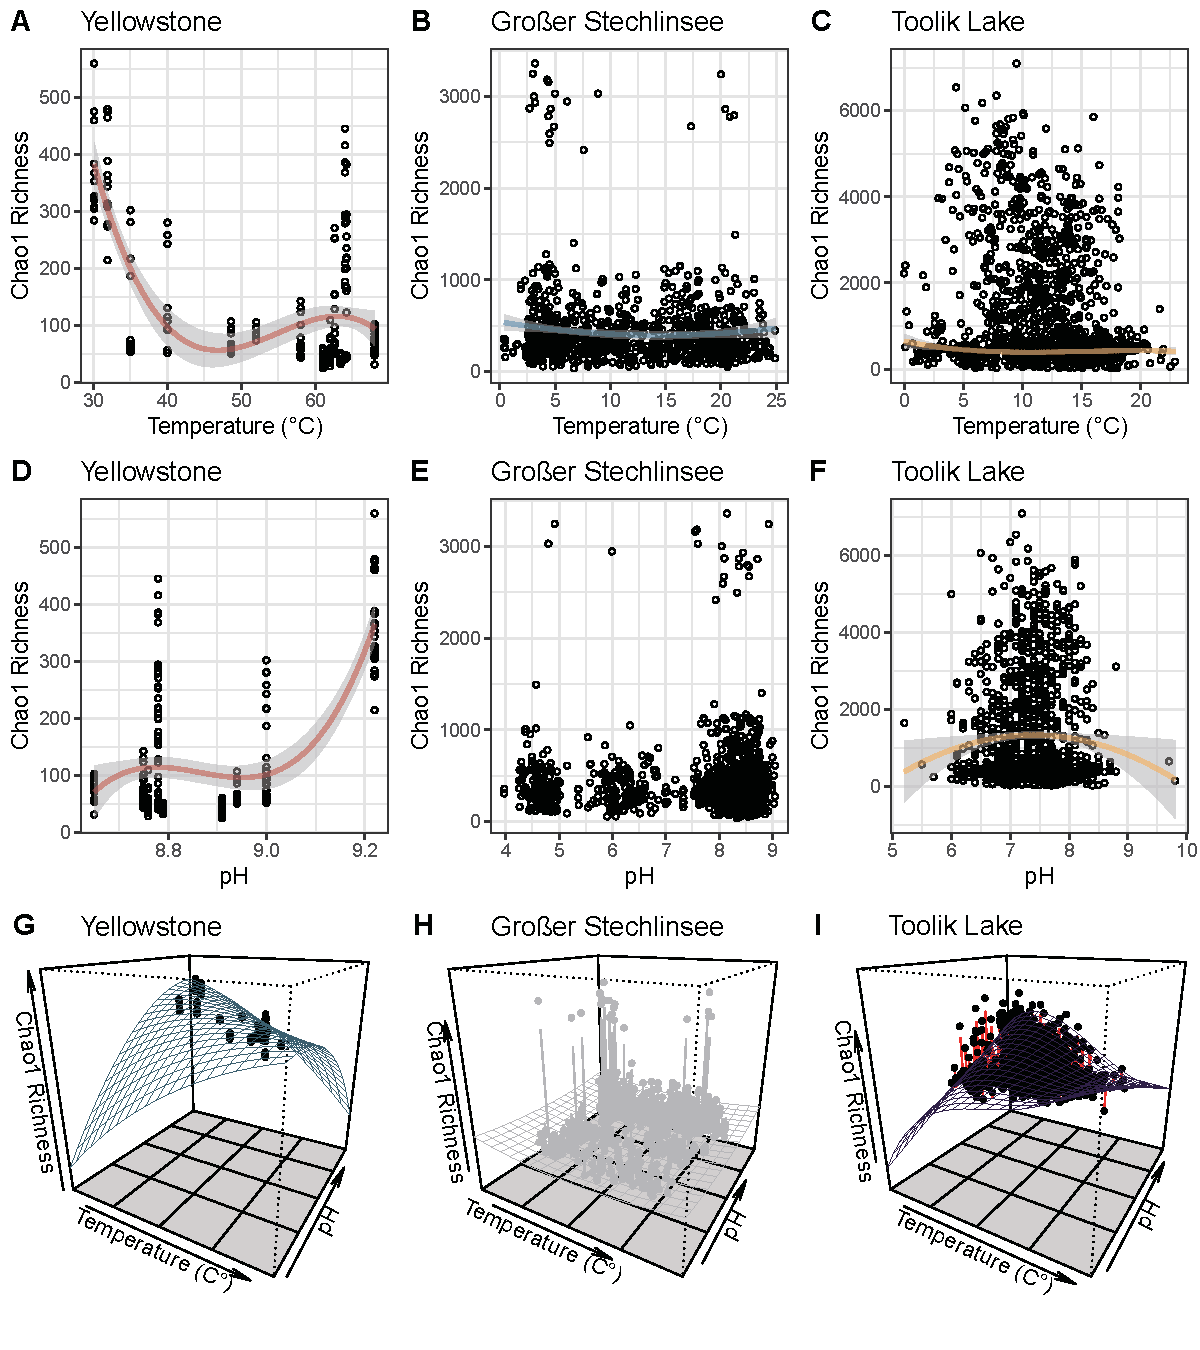
\includegraphics[scale=0.8]{./Figures/Chao_PM_local_1and2EVs_3D}
    \caption{\textbf{Effect of environmental variables on Chao1 richness at the local scale.} A-C: Polynomial regression models of diversity and temperature from three locations ($R^{2}$=0.473, 0.004, 0.065). D-E: Models of diversity and pH ($R^{2}$=0.289, 0.0363). F: There is no significant relationship between pH and diversity in the Toolik Lake samples. D $\&$ F: Models of diversity and pH ($R^{2}$=0.4996, 0.0025). E: There is no significant relationship between pH and diversity in the Großer Stechlinsee samples. G $\&$ I: Polynomial regression model of diversity versus temperature and pH from local data sets ($R^{2}$=0.433, 0.082). H: There is no significant relationship between environmental variables and richness in the Großer Stechlinsee  samples. As with Shannon diversity, there is still one site dataset that shows no relationship between Chao1 richness and pH, suggesting that pH has little effect on bacterial diversity and temperature is probably the best environmental variable at the local scale, even if the pattern is weak.}
    \label{fig:Chao_PM_local_1and2EVs}
\end{figure}

\begin{figure}[H]
    \centering
    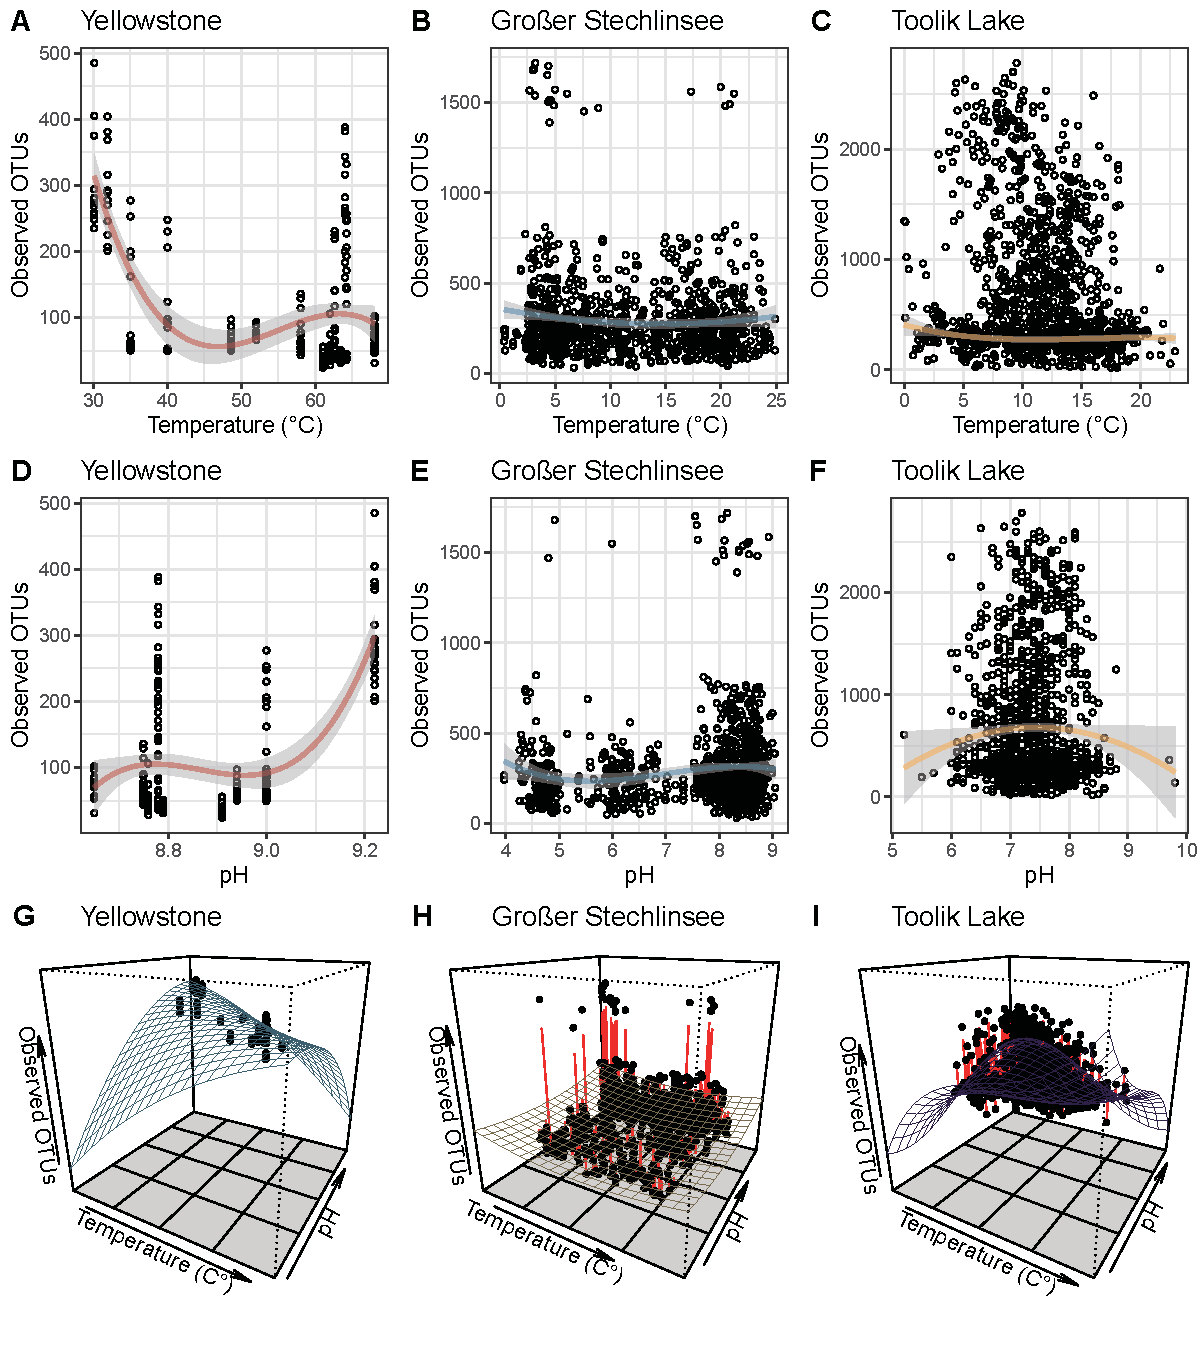
\includegraphics[scale=0.8]{./Figures/OO_PM_local_1and2EVs_3D}
    \caption{\textbf{Effect of environmental variables on absolute species richness (observed OTUs) at the local scale.} A-C: Polynomial regression models of diversity and temperature from three locations ($R^{2}$=0.473, 0.004, 0.065). D-F: Models of diversity and pH ($R^{2}$=0.437, 0.01, 0.002). G-I: Polynomial regression model of richness versus temperature and pH from three location data sets ($R^{2}$=0.433, 0.014, 0.082). Patterns of environmental variables and richness can be found for all data sets, and the data fit is better than the other two indices. These results show similar results to diversity at the local scale.}
    \label{fig:OO_PM_local_1and2EVs}
\end{figure}

\end{document}